%
%  fi_lib++  --- A fast interval library (Version 2.0)                     
%                                                                  
%  Copyright (C) 2001:                                                        
%                                                     
%  Werner Hofschuster, Walter Kraemer                               
%  Wissenschaftliches Rechnen/Softwaretechnologie (WRSWT)  
%  Universitaet Wuppertal, Germany                                           
%  Michael Lerch, German Tischler, Juergen Wolff von Gudenberg       
%  Institut fuer Informatik                                         
%  Universitaet Wuerzburg, Germany                                           
% 
%  This library is free software; you can redistribute it and/or
%  modify it under the terms of the GNU Library General Public
%  License as published by the Free Software Foundation; either
%  version 2 of the License, or (at your option) any later version.
%
%  This library is distributed in the hope that it will be useful,
%  but WITHOUT ANY WARRANTY; without even the implied warranty of
%  MERCHANTABILITY or FITNESS FOR A PARTICULAR PURPOSE.  See the GNU
%  Library General Public License for more details.
%
%  You should have received a copy of the GNU Library General Public
%  License along with this library; if not, write to the Free
%  Foundation, Inc., 59 Temple Place, Suite 330, Boston, MA  02111-1307 USA
%


\documentclass{report}
%\usepackage{a4wide}
\usepackage{amssymb}
\usepackage{amsmath}
%\usepackage{epsfig}
\usepackage[dvips]{graphics}

%\usepackage{listings}

\textwidth      13.0cm
\textheight     20.1cm
\topmargin       0.0cm
\evensidemargin  3cm
\oddsidemargin   0cm
\parindent 0pt

\newcommand{\Rs}{\mathbb{R}^*}
\newcommand{\R}{\mathbb{R}}
\newcommand{\IR}{\mathbb{IR}}
\newcommand{\IRs}{\mathbb{IR}^*}
\newcommand{\xx}{\mathbf{x}}
\newcommand{\ffs}{\mathbf{f}^*}
\newcommand{\ff}{\mathbf{f}}
\newcommand{\INFTY}{\texttt{INFTY}}
\newtheorem{defin}{Definition}
\newtheorem{theorem}{Theorem}
\newcommand{\Pot} {\mbox{\raisebox{0.4ex}{\boldmath $\wp$}} }
\newcommand{\url}[1]{{\small\texttt{#1}}}

\newcommand{\EpsPicScaled}[2]{
  \begin{center}
    \leavevmode
    \renewcommand{\epsfsize}[2]{#2##1}
    \epsffile{#1.eps}
  \end{center}
}
\begin{document}
\begin{titlepage}
\setcounter{page}{0}

\vspace*{5cm}

% Kommentar

\hspace{2.25cm}
\begin{minipage}{11.6cm}
\begin{center}
{\LARGE\bf \texttt{filib++} -   Interval Library \\
	  Specification and Reference Manual\\ }

\vspace*{0.9cm}

{\Large\sf Michael Lerch, German Tischler,\\ J\"urgen Wolff von Gudenberg}

\vspace*{1cm}

\hspace*{1.5cm} Report No.\ ??? \hfill March 2003 \hspace*{1.5cm} 


\vspace*{4.5cm}
Lehrstuhl f\"ur Informatik II\\
Universit\"at W\"urzburg\\
Am Hubland\\
97074 W\"urzburg\\[3mm]
{\tt \{wolff\}@informatik.uni-wuerzburg.de}
\end{center}
\vspace*{2cm}
Parts of this report have
	  been published in \cite{rnc, multi}
\end{minipage}

\end{titlepage}

\tableofcontents
\pagebreak
\section*{Abstract}
\texttt{filib++} is an extension of the interval library \texttt{filib}
originally developed in Karlruhe \cite{filib}. The most important aim of the
latter was the fast computation of guaranteed bounds for interval versions of a
comprehensive set of elementary function. \texttt{filib++} extends this library
in two aspects. First, it adds a second mode, the "extended" mode, that
extends the exception-free computation mode using special values to represent
infinities and NotaNumber known from the IEEE floating-point standard 754 to
intervals. In this mode so-called  containment sets are computed to enclose the
topological closure of a range of a function defined over an interval
\cite{ext}. Second, state of the art design uses templates and traits classes
in order to get an efficient, easily extendable and protable library, fully
according to the C++ standard \cite{c++}.

\section*{Overview}
Chapter 1 presents the difference between the normal mode computing interval
evaluations and the extend mode computing containment sets. The functionality
of the library is roughly sketched.

Chapter 2 then shortly explains the inner structure and describes how to use
it. Some sample programs are listed.

Chapters 3,4,5 contain the specification of the complete interface.

Finally, chapter 6 gives some installation hints.

	\chapter{Interval Evaluation and Containment Evaluation}
	\section{Interval Evaluation}	
We assume that the reader is familiar with the basic ideas of interval
arithmetic. In this introductory chapter we use bold face for
continuous intervals, represented by two real bounds.
\[ \xx = [\underline{x},\overline{x}] = \{ x \in \R |\underline{x} \le x \le
\overline{x}\} \] 
$\IR$ denotes the space of all finite intervals.

%%In this section we shortly summarize the ideas of  \cite{sun,ext}.
Let us deal with the enclosure of a range of a function, one of the main topics
of interval arithmetic. We restrict our consideration to the one-dimensional
case, extensions to more dimensions are obvious.
 Given an arithmetic function $f : D_f \subseteq \R \rightarrow \R$,
$f(\xx)$ denotes the range of values of $f$ over the interval $\xx \subseteq
D_f$. 
\begin{defin}:\\  The \textbf{interval evaluation} $\ff: \IR \rightarrow \IR$ of $f$ is defined as the
function that is obtained by replacing every occurence of the variable $x$ by
the interval variable $\xx$ and by replacing every operator by its
interval arithmetic counterpart and every elementary function by 
 its range. Note, that this definition only holds, if all
operations are executable without exception.
\end{defin}


The following theorem is known as the fundamental theorem of interval
arithmetic.
\begin{theorem}:\\
If the interval evaluation is defined, we have
\[ f(\xx) \subseteq \ff(\xx) \]
\end{theorem}

The interval evaluation is not defined, if $\xx$ contains a point $y
\notin D_f$. Division by an interval containing 0, e.g., is forbidden.
But note, that even if $\xx \subseteq D_f$, $\ff$ may  not be defined. The result
depends on the syntactic formulation of the expression.


%%\textbf{counter example:} 
$f_1(x) = \frac{1}{x\cdot x + 2} $\\
$ \mathbf{f}_1([-2,2])$
is not defined, because
 $[-2,2] \cdot [-2,2] = [-4,4]$

whereas
 $ f_2(x) =
\frac{1}{x^2 +2}$\\ yields  $\mathbf{f}_2([-2,2])= [1/6, 1/2]$.

%%%%  5.2.02 %%%
The elementary functions $f$ are defined as the set  of all function values,
that is an  interval,
because the functions are continuous over their domain. 
That means that  the interval evaluation is
equal to the range, if it is defined. The interval evaluation is not defined,
if the argument interval contains a point outside the domain of the
corresponding function.
%%%%  5.2.02 %%%

$\ff(\xx):= f(\xx) = \{f(x)| x \in \xx \subseteq D_f\}$



\section{Containment Evaluation}


To overcome the difficulties with partially defined functions throwing
exceptions, we introduce a second mode, the ``extended'' mode.
Here, usually no exceptions are raised, but the domains of interval
functions and  ranges of interval results are consistently extended.

Following G. W. Walster in \cite{sun,ext} we define the containment set:
\begin{defin}:\\
Let $f : D_f \subseteq \R \rightarrow \R$, then the containment set
$f^\ast: \Pot\R^\ast\mapsto \Pot\R^\ast$ defined by
\begin{equation}
f^*(\xx):= \{f(x)| x \in \xx \cap D_f\} \cup \{ \lim_{x\rightarrow x^*} f(x) | x
\in D_f, x^* \in \xx\} \subseteq \Rs   \label{cs}
\end{equation} contains the extended range of $f$, where
$\Rs = \R \cup \{ -\infty\} \cup \{ \infty\}$.
\end{defin}

Hence, the containment set of a function is the closure of the range including all
limits and accumulation points.

Our goal is now to define an analogon to the interval evaluation which encloses
the containment set, and is easy to compute.

Let $\IRs$ denote the set of all extendeded intervals with endpoints in $\Rs$ .

\begin{defin}:\\  The \textbf{containment evaluation} $\ffs: \IRs \rightarrow \IRs$ of $f$ is defined as the
function that is obtained by replacing every occurence of the variable $x$ by
the interval variable $\xx$ and by replacing every operator  or function by its
extended interval arithmetic counterpart.
\end{defin}

We then have
\begin{theorem}:\\
The containment evaluation is always defined, and we have
\[ f^*(\xx) \subseteq \ffs(\xx) \]
\end{theorem}

For the proof of this theorem all arithmetic operators and elementary functions
are extended to the closure 
of their domain. This can be done in a straight
forward manner, cf. \cite{sun}. We apply the well known rules to compute with
infinities. If we encounter an undefined operation like $ 0 \cdot \infty$ we
deliver the set of all limits, i.e. $\Rs$. Note that negative values are also
possible, since 0 can be approached from both sides.

We show the containment sets for the basic arithmetic operations in
the following tables.


\begin{table}
\[
\begin{array}{l|ccc}
\hline
+&-\infty & y &+\infty\\
\hline
-\infty  & -\infty & -\infty &\Rs\\
x   &   -\infty  & x+y     &     +\infty\\ 
+\infty &  \Rs & +\infty & +\infty\\
\hline
\end{array}
\]
\caption{\label{add}extended addition}
\end{table}

\begin{center}
\begin{table}
\[
\begin{array}[t]{l|ccc}
\hline
-&-\infty & y &+\infty\\
\hline
-\infty  &\Rs& -\infty & -\infty \\
x   &   +\infty  & x-y     &     -\infty\\ 
+\infty & +\infty & +\infty &  \Rs\\
\hline
\end{array}
\]
\caption{\label{sub}extended subtraction}
\end{table}
\end{center}

\begin{center}
\begin{table}[!]
\[
\begin{array}{l|ccccc}
\hline
*&-\infty & y<0&0&y>0 &+\infty\\
\hline
-\infty  & +\infty & +\infty &\Rs& -\infty & -\infty\\
x <0  &   +\infty  & x*y   &0&x*y&     -\infty\\
0& \Rs & 0 &0 &0& \Rs\\ 
x >0  &   -\infty  & x*y   &0&x*y&     +\infty\\
+\infty & -\infty & -\infty& \Rs & +\infty & +\infty\\
\hline
\end{array}
\]
\caption{\label{mul}extended multiplication}
\end{table}
\end{center}

\begin{center}
\begin{table}[!]
\[
\begin{array}{l|ccccc}
\hline
/&-\infty & y<0&0&y>0 &+\infty\\
\hline
-\infty  & [0,+\infty] & +\infty & \{-\infty ,+\infty\}& -\infty & [-\infty,0]\\
x < 0  & 0&  x/y & \{-\infty ,+\infty\} &x/y&0\\
0& 0& 0  &\Rs &0 &0\\ 
x >0  &   0  & x/y   &\{-\infty, +\infty\}&x/y&     0\\
+\infty & [-\infty,0]& -\infty& \{-\infty ,+\infty\} & +\infty & [0,+\infty] \\
\hline 
\end{array}
\]
\caption{\label{div}extended division}
\end{table}
\end{center}

From these tables the definition of extended interval arithmetic can easily be
deduced. For addition, subtraction, and multiplication can be returned, if a
corresponding operation is encountered.

Some examples:

$[2, \infty] + [3,\infty] = [5, \infty]$\\
$[2, \infty] - [3,\infty] = \Rs$\\
$[2, \infty] * [-3,3] =\Rs$\\

Division is a little bit more subtle. Table \ref{idiv} shows the cases where
the denominator contains 0.

\begin{center}
\begin{table}[!]
\[
\begin{array}{llll}
\hline
A=[\underline{a};\overline{a}]&B=[\underline{b};\overline{b}]&
\textrm{Range}&\textrm{containment set}\\
\hline
0\in A&0\in B&\R^\ast&\R^\ast\\
0\in
A&B=[0;0]&\{-\infty;+\infty\}&\R^\ast\\
\overline{a}<0&\underline{b}<\overline{b}=0&[\overline{a}/\underline{b},\infty)&[\overline{a}/\underline{b},\infty]\\
\overline{a}<0&\underline{b}<0<\overline{b}&(-\infty;\overline{a}/\overline{b}]\cup[\overline{a}/\underline{b},+\infty)&\R^\ast\\
\overline{a}<0&0=\underline{b}<\overline{b}&(-\infty;\overline{a}/\overline{b}]&[-\infty;\overline{a}/\overline{b}]\\
\underline{a}>0&\underline{b}<\overline{b}=0&(-\infty;\underline{a}/\underline{b}]&[-\infty;\underline{a}/\underline{b}]\\
\underline{a}>0&\underline{b}<0=\overline{b}&(-\infty;\underline{a}/\underline{b}]\cup[\underline{a}/\overline{b},+\infty)&\R^\ast\\
\underline{a}>0&0=\underline{b}<\overline{b}&[\underline{a}/\overline{b};+\infty)&[\underline{a}/\overline{b};+\infty]
\end{array}
\]
\caption{\label{idiv}extended interval division}
\end{table}
\end{center}




For the elementary functions Table \ref{sf} shows the extended
domains and extended ranges.


\begin{table}
\begin{tabular}{llll}
\hline
name& domain & range &special values\\
\hline
sqr & $\Rs$ & $[0,\infty]$ &\\
power &$\Rs \times \mathbb{Z}$ & $\Rs$&power([0,0],0) = [1,1]\\ 
pow &$ [0,\infty]\times \Rs$ & $[0,\infty]$&pow([0,0],[0,0]) =$[0,\infty]$ \\ 
sqrt & $[0,\infty]$& $[0,\infty]$ &\\
exp, exp10, exp2 &  $\Rs$ & $[0,\infty]$ &\\
expm1&  $\Rs$ & $[-1,\infty]$ &\\
log, log10, log2 & $[0,\infty]$&$\Rs$&log $( [0,0]) = [-\infty]$\\ 
log1p &$[-1,\infty]$ &$\Rs$&log1p $( [-1,-1]) = [-\infty]$\\
 \hline
sin& $\Rs$& $[-1,1]$&\\
cos& $\Rs$& $[-1,1]$&\\
tan& $\Rs$& $\Rs$& tan($\xx$) = $\Rs$, if\\
&&&$\pi/2 + k\pi \in \xx, k\in \mathbb{Z}$\\
cot& $\Rs$& $\Rs$& cot($\xx$) = $\Rs$, if\\
&&&$ k\pi \in \xx, k\in \mathbb{Z}$\\
asin& $[-1,1]$&$[-\pi/2,\pi/2]$&\\
acos& $[-1,1]$&$[0,\pi]$&\\
atan& $\Rs$&$[-\pi/2,\pi/2]$&\\
acot& $\Rs$&$[0,\pi]$&\\ \hline
sinh& $\Rs$&$\Rs$&\\
cosh&$\Rs$&$[1,\infty]$&\\
tanh &$\Rs$&$[-1,1]$&\\
coth&$\Rs$&$[-\infty,-1]\cup[1,\infty]$&coth[0,0] =$\Rs$\\ 
asinh& $\Rs$&$\Rs$&\\
acosh&$[1,\infty]$&$[0,\infty]$&\\
atanh &$[-1,1]$&$\Rs$&\\
acoth&$[-\infty,-1]\cup[1,\infty]$&$\Rs$&acoth$[-1,-1]=[-\infty]$\\
&&&acoth$[1,1]=[\infty]$\\
\hline
\end{tabular}
\caption{\label{sf} extended domains and ranges of elementary functions}
\end{table}

%%%%  5.2.02 %%%
The containment evaluation for an elementary function is computed by directly
applying the definition of the containment set.
\begin{quote}
$\ff^*(\xx):= \Diamond(  \{f(x)| x \in \xx \cap D_f\}  \cup \{ \lim_{x\rightarrow x^*} f(x) | x
\in D_f, x^* \in \xx\} )$

Here $\Diamond$ denotes the interval hull.
%%%%  5.2.02 %%%

 If the argument lies strictly outside
the domain of the function, we obtain the empty set as result.

If the argument $\xx$ contains a singularity the corresponding values
for $\pm \infty$ are produced.

The functions in containment mode never produce an overflow or illegal argument error.
\end{quote}


Some examples:

$\log[-1,1] = [-\infty,0] $, $\sqrt{[-1,1]} = [0,1]$, $\log[-2,-1]=\emptyset$, $\coth[-1,1]=\R^\ast$\\

The special values column shows the results of the interval version at points
		on the border of the open domain. In all cases the lim construction in (\ref{cs})
		is applied and containment is guaranteed. Note that for the
		power  function $x^k$ only
		$\lim_{x \rightarrow 0} x^0 $ is to be considered whereas $x^y$ is calculated
		as $e^{y \ln x}$ in the pow function. We intentionally chose 2
		different names, since power$(\xx,k) \subseteq $
		pow$(\xx,[k,k])$ does not hold for negative $\xx$.

It has been shown in \cite{ext,simple}, that using these extended operations
 the containment evaluation can be
computed without exceptions.


\section{Functional Specification of \texttt{filib++} -- Overview}
\subsection{Internal Representation}
\label{intrep}

In the normal mode of the library continuous real intervals are represented by
two floating-point bounds, in fact a more general instantiation is possible,
see \ref{template}.
If a function or interval evaluation is not defined, the  exception
handling  for the floating-point type is activated. That should terminate the
program with an error message.


To cope with the closed set of real numbers in the extended mode, we accept the
IEEE representation 
of $-\infty$, or  $\infty$  as left or right hand
bound of an extended interval, respectively. Thus we introduce one-sided open
intervals: 
\[ \xx = [\underline{x},\infty] = \{ x \in \R | x \ge\underline{x}\} \]
\[ \xx = [-\infty,\overline{x}] = \{ x \in \R | x \le\overline{x}\} \]
The real numbers larger than the overflow threshold \verb|M| are
\[ \xx = [ \verb|M|,\infty] = \{ x \in \R | x \ge \verb|M|\} \]
\[ \xx = [-\infty,\verb|-M|] = \{ x \in \R | x \le\verb|-M|\} \].
\[
 [-\infty,\infty] = R^*\] means all numbers.

The emtpy interval
$\emptyset$  is represented as $[$\verb|NaN,NaN|$]$ .
There are, however, no point
intervals  $[-\infty$,   $-\infty]$ or $[\infty$,   $\infty]$, we use the
closed exterior intervals
instead. This trick helps in a clear set theoretical interpretation and also
facilitates the implementation. If we consider $R^*$ as the base set all the
open intervals can be interpreted as closed, and the usual formulae for
interval arithmetic extended with obvious rules for $\pm \infty$ can be
applied. 

\subsection{Construction and Access}
The interval constructor expects two or one floating-point values
as arguments with a default
value for the point interval [0.0, 0.0]. Inf and sup are accessible via
methods. There are checks for point interval (\verb|isPoint|), empty interval
(\verb|isEmpty|) and unbounded interval  (\verb|isInfinite|). To check for
sharpness of an interval the method  \verb|hasUlpAcc(n)| is provided, it is
fulfilled, if both bounds differ at most by n ulps (unit last place).
 
\subsection{Arithmetic Operations}
The extended arithmetic operations for this data type, abbreviated as \verb|I|
and the base type \verb|double| = \verb|D| are accessible as overloaded
operators. Operand combinations \verb|I x I| \verb|D x I|, and \verb|I x D| are
available for all operations $+, -, *, /$.
Assignment
operators $+=,-=,*=,/=$ are provided for  \verb|I x I| and \verb|I x D| as
methods of the class \texttt{interval}.


\subsection{Relations}
All 3 kinds of set-like, certainly or possibly comparisons \cite{sun} are
provided as methods and as functions.
 The operators \verb|==, !=, >=, <=| are overloaded for
the set-like relations. We further supply the predicate  $y\ \verb|interior|
\ \xx \iff \underline{x}<y<\overline{x}$. 

\subsection{Set Theoretic Functions}
Utility methods and functions  like midpoint, radius, diameter of an interval, its
mignitude or magnitude, the interval of all absolute values, minima, maxima are
provided. Lattice operations as intersection  (\verb|intersect|) or interval
 hull  (\verb|hull|)can be performed
and the Hausdorff distance  (\verb|dist|) between  two intervals can be
computed. 

\subsection{Elementary Arithmetic Functions}
 The provided elementary functions and their (closed) domains and ranges
are listed in table \ref{sf}. In the normal mode the true domains of
the functions are valid, i.e. log$[0,1.0]$ yields an error. 
The implemented elementary functions do not return least-bit accurate
results, but an almost enclosure within a few ulps
 of the range is always guaranteed.
 \subsection{Input and Output}
The standard input output operators are overloaded for intervals, but without
appropriate rounding to the external decimal string format.



	\chapter{Instantiation and Options}
		\section{Namespace filib}

The library is contained in the namespace
		\texttt{filib}. Hence, it is required to qualify each
		identifier of the library with \texttt{filib::}
		or to use the directive
		\texttt{using namespace filib}.

		\section{Two Modes}
In the default or ``normal'' mode traditional interval
evaluations are computed, and the program terminates, if the argument
interval is not contained in the domain of a function.
Overflow treatment is done according to the chosen floating point option.

In the ``extended'' mode containment sets over $\Rs$ are computed, no
exceptions are raised. This mode is obtained by setting a template parameter
accordingly.

Normal mode intervals and extended mode intervals can be used within the same
program without recompilation of the code.
		
		\section{Template Parameters of Class
		\texttt{interval<>}} \label{template}
An interval is defined as a template.
There are 3 template parameters, the underlying basic
		(floating-point) number type
		\texttt{N}, the method, how to implement the directed
		roundings \texttt{rounding\_control} and the mode.

		\subsection{Basic Number Type}
		\label{Zahlentyp}

An interval is given by 2 computer representable bounds, the lower
bound or infimum and the upper bound or supremum 

\[ \xx = [\underline{x},\overline{x}] \]

It represents the continous set of all numbers from the mathematical
set $\mathbb{S}$ that is approximated by the basic number type
\texttt{N}, e.g. $\S=\R$ and \texttt{N}=\texttt{double}.

\[ \xx = [\underline{x},\overline{x}] = \{x \in \mathbb{S}
|\underline{x} \leq x \leq \overline{x} \} \]

The type \texttt{N} has to be an arithmetic type, i.e. all the
operators have to be provided. In the extended mode constants for
 $\pm\infty$ und \texttt{NaN} are needed. These constants are supplied
 by the \texttt{fp\_traits<>} class.
Currently the only reasonable choices are  \texttt{double} or
\texttt{float}. Hence,  only $\mathbb{R}$ can be taken for $\mathbb{S}$. 
The elementary functions for a basic type  cannot be
generated by instantiation of a template, but have to be implemented
by suitable algorithms. In the current version of \texttt{filib++} only
\texttt{double} functions are implemented. \footnote{this
implementation is the original \texttt{filib} code, see \cite{filib}}



		\subsection{Rounding Control}
		\label{Rundungskontrolle}


Rounding, the use of the directed roundings in particular, is
controlled by the second template parameter. It
addresses the low-level, machine dependent part of the
implementation.

The second parameter can have the following values
\begin{itemize}

\item \textit{native\_switched:}
Before an operation computing a  floating-point bound of the interval 
is executed, the rounding mode is
switched via an 
assembler statement that changes the 
floating-point control word. This is an expensive operation, since the
pipelines have to be cleared. After the interval operation the
rounding mode is switched back to the default. This is our default mode for
interval operations.
\item \textit{native\_directed:}
The same as \textit{native\_switched} but the rounding mode is not
switched back. Note, that this mode influences the non-interval
operations of the program.
\item \textit{multiplicative:}
If the architecture does not support directed rounding modes, they can be
simulated by a multiplication of the result.

We define two functions ($R$ is a floating-point screen):

 $\mathrm{low} : R \rightarrow R$
\begin{equation}
\mathrm{low}(a):=\left\{
\begin{array}{ll}
a\ge 0: & a\odot \textrm{pred}(1) \\
%a=0: & \textrm{pred}(0) \\
a<0: & a\odot \textrm{succ}(1)
\end{array}
\right.
\label{low}
\end{equation}
and $\mathrm{high} : R \rightarrow R$ 
\begin{equation}
\mathrm{high}(a):=\left\{
\begin{array}{ll}
a\ge 0: & a\odot \textrm{succ}(1) \\
%a=0: & \textrm{succ}(0) \\
a<0: & a\odot \textrm{pred}(1).
\end{array}
\right.
\label{high}
\end{equation}
where $\odot$ means \emph{round-to-nearest}-multiplication and where
$\mathrm{succ}(x) = \mathrm{min}\{y|y \in R, y > x\}$ or 
$\mathrm{pred}(x) = \mathrm{max}\{y|y \in R, y <x\}$, respectively.



Note that, because $\mathrm{high}(a) = -\mathrm{low}(-a)$, one function
suffices. 

For a binary floating-point system $R=R(2,n,emin,emax)$ we have 
\[\mathrm{pred}(1) = 1 -2^{-n} = 1 - \frac{1}{2}\varepsilon ^*\]
\[\mathrm{succ}(1) = 1 +2^{1-n} = 1 + \varepsilon ^*\]
where $\varepsilon ^* = 2^{1-n}$ denotes the bound for the relative rounding
error 
($|\varepsilon| \le \varepsilon^*$).

\begin{theorem}:\\
Let  $R=R(2,n,emin,emax)$ be  a binary floating-point system and $\bigcirc :
\R \rightarrow R$ the rounding to the nearest. Then for all $x \in \R$ not
in the over- or underflow range, i.e. $\verb?M? \ge |x| \ge 2^{emin-1}$ or $x = 0$, we have 
\[  \mathrm{low}(\bigcirc x) \le x \]
\[  \mathrm{high}(\bigcirc x) \ge x \]
\end{theorem}

For the proof, see \cite{multi}.
\item \textit{pred\_succ\_rounding:}
Another way to simulate the directed roundings is to manipulate the
representation of a floating-point number in order to obtain the predecessor or
successor of that number. This is usually done using integer arithmetic. It can
be sped up, if a table of $\textrm{ulp}(x)$ is stored containing the unit in last
place with respect to the exponent of $x$.

		\item \textit{no\_rounding:} 
This mode is only for testing and tuning. Do NOT use it in
applications. It does NOT compute enclosures.
\end{itemize}

The one-sided rounding mode seems to be very appealing, since it minimizes
switches of the rounding control. But note, that it currently does not work in
the case 
of gradual underflow. For i386 architectures the rounding of values in the
overflow range to $\pm \infty$ have to be forced by an intermediate storing of
the value and, hence, the predicted performance gain is lost.

IMPORTANT: it is necessary to call the method 
\begin{center}
	\texttt{filib::fp\_traits<N,K>::setup()}
\end{center}
whenever you use instances of a different instantiation of the \texttt{interval<>}
class with template parameters \texttt{N,K}. This is especially true
at program start. 
		\subsection{Mode}
		\label{Modus}

The mode parameter can have the following values (see \ref{intrep}):

\begin{itemize}
\item[] \texttt{filib::i\_mode\_normal}: normal evalutation with program termination
at illegal operations
\item[] \texttt{filib::i\_mode\_extended}: extended exception free evaluation
\item[] \texttt{filib::i\_mode\_extended\_flag}: extended exception free evaluation where
the exception flag is set if the normal mode would produce an error
\end{itemize}

\section{Traits}

Let us have a closer look into the design of the library.  The
\texttt{interval<>} class  implements its operations relying on functions for
directed floating-point arithmetic operations and on a function to reset the
rounding mode. For example a simplified version of the \texttt{+=}
operator looks like:

\begin{verbatim}
interval<N,K,E> & interval<N,K,E>::operator +=
(interval<N,K,E> const & o)
{
  INF=fp_traits<N,K>::downward_plus(INF,o.INF);
  SUP=fp_traits<N,K>::upward_plus(SUP,o.SUP);
  fp_traits<N,K>::reset();
  return *this;
}
\end{verbatim}


 These type and rounding mode specific  operations are provided by a traits class
\texttt{fp\_traits<>} that handles all the operations depending on the type \texttt{N} and
rounding control \texttt{K}. Specializations of this traits class for \texttt{double} and
\texttt{float} and each of the described rounding control mechanisms
   are instantiated in the library. The specializations for rounding modes that
rely on machine specific rounding control methods inherit these methods from an
instantiation of the class \texttt{rounding\_control}. That is illustrated in the
following diagram.

\begin{figure}
\begin{center}
\resizebox{11cm}{!}{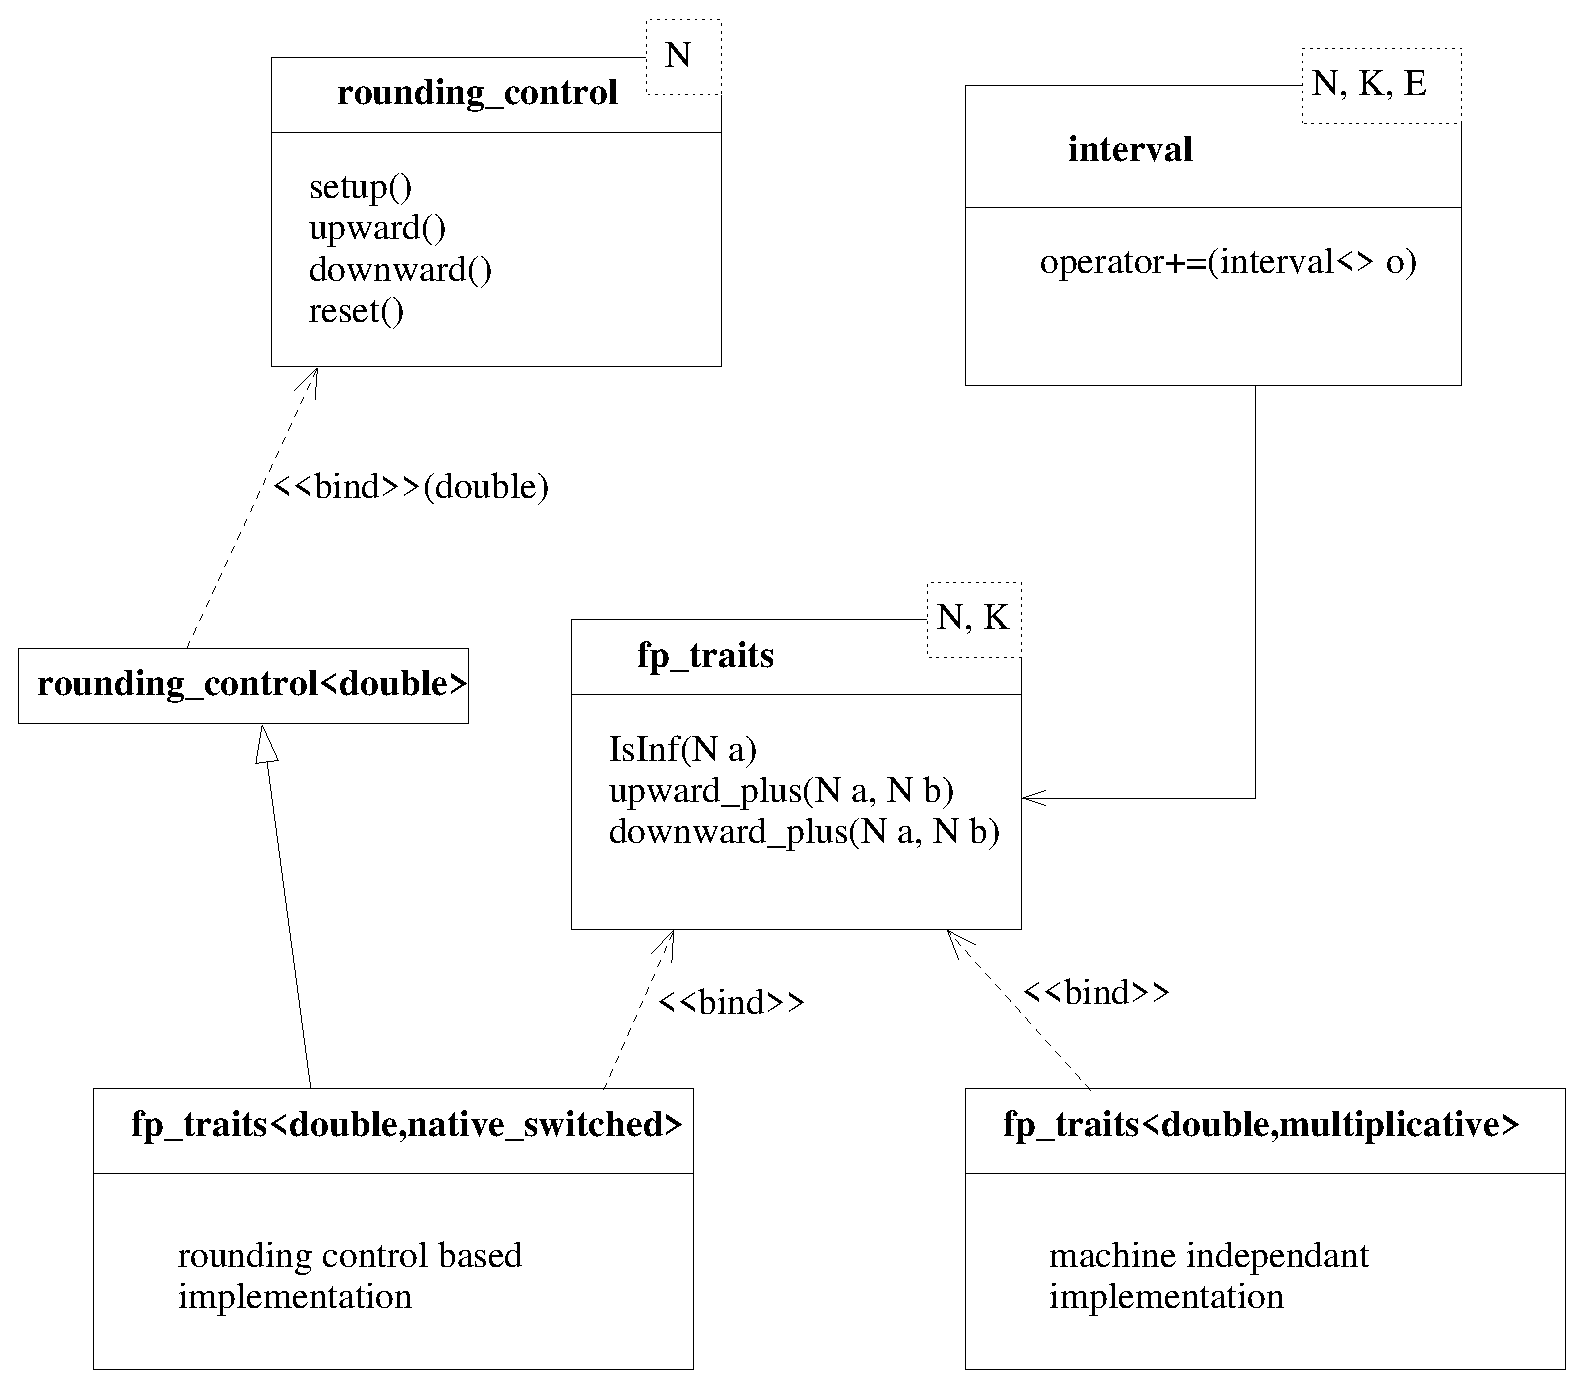
\includegraphics{traits}}
\end{center}
\end{figure}
%\EpsPicScaled{traits}{0.45}

\section{Instantiation Examples}
	Some examples may help to use the library. Another example
can be found in the \texttt{examples} directory of the distribution.
		\begin{itemize}
		
			\item \texttt{filib::interval<double> A;}\\
This is the default instantiation.
				\texttt{A} is an  interval over the
		floating-point type
				\texttt{double}. The second and third parameter
		are set to their defaults
\textit{filib::native\_switched} and
\textit{filib::i\_mode\_normal}

			\item \texttt{filib::interval<double,filib::multiplicative> A;}\\
				\texttt{A} is an  interval over
				 \texttt{double}.  Multiplicative
				rounding is used. The hardware need
				not support directed roundings.

			\item \texttt{filib::interval<double,filib::native\_switched,filib::i\_mode\_extended> A;}\\
				\texttt{A} is an  interval over the
		floating-point type \texttt{double}. It uses 
    \textit{filib::native\_switched} for rounding and is treated as an extended interval.
		\end{itemize}

\section{Sample Programs}
	
		\subsection{Evaluation of a Polynomial -- Template Version}
	%		\lstset{labelstyle=\normalsize,labelstep=1,labelsep=8pt,indent=15pt}
%%			\begin{lstlisting}{}
\begin{verbatim}
// Simple usage of the library filib++ (template version)
 
#include <interval/interval.hpp>
#include <vector> // STL container vector
#include <iostream>

using filib::interval;
using std::vector;
using std::cout;
using std::endl;

// Evaluation of a polynomial using Horner's rule 
interval<double> horner
(
   // interval coefficients in STL container vector 
   vector< interval<double> > const & pol, 
   // interval argument   
   interval<double> x 
)
{
   // result 
   interval<double> res = interval<double>();  // res is [0,0]

   vector< interval<double> >::const_iterator p= pol.begin();

   while ( p != pol.end() )
   {
      res *= x; 
      res += *(p++);
   }
   return res; // now res == pol(x)
 }

int main()
{
   filib::fp_traits<double>::setup();
   interval<double> coeff2(2), coeff1(5), coeff0(3), x(2,4);
   vector< interval<double> > pol; 
   pol.push_back(coeff2); 
   pol.push_back(coeff1);
   pol.push_back(coeff0);
   // horner(pol,x) computes coeff2*x*x + coeff1*x + coeff0
   cout << "pol(x)= " << horner(pol,x) << endl;
   interval<double> y(-1,1); 
   cout << "pol(y)= " << horner(pol,y) << endl;
   return 0;
}
\end{verbatim}
%%\end{lstlisting}

	\chapter{The \texttt{fp\_traits<>} class}
	\section{Template Arguments}
	The \texttt{fp\_traits<>} class is a template class with
	two template arguments. The first argument is supposed
	to be a numeric type, where there are currently implementations
	for \texttt{float} and \texttt{double}. The second parameter
	is a non-type parameter of type \texttt{rounding\_strategy}
	as described in section \ref{Rundungskontrolle}. The following table
	shows the  currently available combinations.

	\begin{center}
	\begin{tabular}{|l|l|}
	\hline
	first param&second param\\
	\hline\hline
	\texttt{double}&\texttt{native\_switched}\\
	\hline
	\texttt{double}&\texttt{native\_directed}\\
	\hline
	\texttt{double}&\texttt{multiplicative}\\
	\hline
	\texttt{double}&\texttt{no\_rounding}\\
	\hline
	\texttt{double}&\texttt{pred\_succ\_rounding}\\
	\hline
	\texttt{float}&\texttt{native\_switched}\\
	\hline
	\texttt{float}&\texttt{native\_directed}\\
	\hline
	\texttt{float}&\texttt{multiplicative}\\
	\hline
	\texttt{float}&\texttt{no\_rounding}\\
	\hline
	\end{tabular}
	\end{center}
\section{Utility Functions}
	The following static member functions are mandatory
	for all implementations of the \texttt{fp\_traits<>}
	class (where \texttt{N} denotes the first template parameter):

	\begin{itemize}
		\item \texttt{bool {\bf IsNaN}(N const \& a)}\\ 
			test if \texttt{a} is not a number
		\item \texttt{bool {\bf IsInf}(N const \& a)}\\
			test if \texttt{a} is infinite
		\item \texttt{N const \& {\bf infinity}()}\\ returns positive infinity
		\item \texttt{N const \& {\bf ninfinity}()}\\ returns negative infinity
		\item \texttt{N const \& {\bf quiet\_NaN}()}\\ returns a quiet
			(non-signalling) {\bf NaN}
		\item \texttt{N const \& {\bf max}()}\\ returns the maximum finite value
			possible for \texttt{N}
		\item \texttt{N const \& {\bf min}()}\\ returns the minimum finite
			positive non-denormalized value possible for \texttt{N}
		\item \texttt{N const \& {\bf l\_pi}()}\\ returns a close lower bound of $\pi$
		\item \texttt{N const \& {\bf u\_pi}()}\\ returns a close upper bound of $\pi$
		\item \texttt{int const \& {\bf precision}()}\\ returns the current
			output precision
		\item \texttt{N {\bf abs}(N const \& a)}\\ returns the absolute
			value of \texttt{a}
		\item \texttt{N {\bf upward\_plus}(N const \& a, N const \& b)}\\
			returns a value of type \texttt{N}.
			It shall be as close to $a+b$ as possible and
			no smaller than $a+b$.
		\item \texttt{N {\bf downward\_plus}(N const \& a, N const \& b)}\\
			returns a value of type \texttt{N}.
			It shall be as close to $a+b$ as possible and
			no bigger than $a+b$.
		\item \texttt{N {\bf upward\_minus}(N const \& a, N const \& b)}\\
			returns a value of type \texttt{N}.
			It shall be as close to $a-b$ as possible and
			no smaller than $a-b$.
		\item \texttt{N {\bf downward\_minus}(N const \& a, N const \& b)}\\ 
			returns a value of type \texttt{N}.
			It shall be as close to $a-b$ as possible and
			no bigger than $a-b$.
		\item \texttt{N {\bf upward\_multiplies}(N const \& a, N const \& b)}\\
			returns a value of type \texttt{N}.
			It shall be as close to $a\cdot b$ as possible and
			no smaller than $a\cdot b$.
		\item \texttt{N {\bf downward\_multiplies}(N const \& a, N const \& b)}\\ 
			returns a value of type \texttt{N}.
			It shall be as close to $a\cdot b$ as possible and
			no bigger than $a\cdot b$.
		\item \texttt{N {\bf upward\_divides}(N const \& a, N const \& b)}\\
			returns a value of type \texttt{N}.
			It shall be as close to $a / b$ as possible and
			no smaller than $a / b$.
		\item \texttt{N {\bf downward\_divides}(N const \& a, N const \& b)}\\ 
			returns a value of type \texttt{N}.
			It shall be as close to $a / b$ as possible and
			no bigger than $a / b$.
	\end{itemize}

	\chapter{The \texttt{interval<>} class}
	Let $\underline{x}$ or $\overline{x}$ denote infimum or 
	supremum of the interval \texttt{X}, the interval \texttt{this*} is written as \texttt{T =}
	$[\underline{t}$ , $\overline{t}]$. \texttt{N} denotes the underlying
	basic number type,
  i.e the type of the bounds (see \ref{Zahlentyp}). 
  Furthermore
			$M$ is the largest representable  number of type
	\texttt{N} and
	$\pm \texttt{INFTY}$ denotes an internal constant for  $\pm \infty$.
			 $[\texttt{NaN},\texttt{NaN}]$
			represents the empty interval where \texttt{NaN}
	denotes an internal representation for ``Not a Number''.

\section{Basic Number Type}
\begin{itemize}
		\item The typename \texttt{value\_type} is defined for the basic
	number type.
		\item The type of traits used by the class is introduced
	as \texttt{traits\_type}.
\end{itemize}

\section{Error flag access}

For the mode i\_mode\_extended\_flag an error flag is introduced. It is set
whenever an operation produces \texttt{NaN}, an overflow, an empty interval or 
calculates a elementary function value for an argument which is not contained
within the domain of the function. These are exactly the cases where the normal
mode would produce an error. They can occur in interval constructors, arithmetic
operations and elementary function evaluation. Note that the flag is only set
for interval operations, it is not used for non interval operations like \texttt{\bf diam()}.

The following functions are provided:

\begin{itemize}
\item \texttt{\bf bool getExtendedErrorFlag()}: returns the current state of the
extended error flag
\item \texttt{\bf void resetExtendedErrorFlag()}: resets the extended error flag
\end{itemize}

	\section{Constructors}
		The following constructors are provided for the interval class:
		\begin{itemize}
		\item \texttt{{\bf interval}()}:\\ The interval $[0,0]$ is constructed.
		\item \texttt{{\bf interval}(N const \& a)}:\\  The interval
	$[a,a]$ is constructed.The point intervals for
			 $+\infty$ and $-\infty$ are given
	by 
			$[M,+\texttt{INFTY}]$ or $[-\texttt{INFTY},-M]$, respectively.


		\item \texttt{{\bf interval}(N const \& a, N const \& b)}:\\
			If $a \leq b$ the interval $[a,b]$ is
	constructed, otherwise the empty interval.

		\item \texttt{{\bf interval}(std::string const \& infs, std::string const \& sups) \\throw(filib::interval\_io\_exception)}:\\
			Construct an interval using the strings \texttt{infs}
and \texttt{sups}. The bounds are first transformed to the primitive
double type by the function \texttt{strtod} and then the predecessor of the infimum and
the successor of the supremum are taken as bounds. This function is provided by the standard, but
the standard does not require it to be optimal.  If the strings cannot be parsed
by \texttt{strtod}, an exception of type \\\texttt{filib::interval\_io\_exception}
is thrown.
	
		\item \texttt{{\bf interval}(interval<> const \& o)}:\\ Copy
			constructor, an interval equal to the interval
			\texttt{o} is constructed.
		\end{itemize}
	\section{Assignment}

		\begin{itemize}
		\item \texttt{interval<> \& {\bf operator=}(interval<> const \& o)}:\\
	The interval \texttt{o} is assigned.
		\end{itemize}
	\section{Arithmetic Methods}
		The following methods are provided for updating arithmetic
		operations. Note that the usual operators are available as
		global functions (see \ref{Funktionen}).
		
		The special cases of the extended mode are not
		explicitly mentioned here, see tables \ref{add},\ref{sub},\ref{mul},\ref{div} for details.
		\begin{itemize}
		\item 
			\texttt{interval<> const \& {\bf operator+}() const} (unary plus):\\
			The unchanged interval is returned.
		\item
			\texttt{interval<> {\bf operator-}() const} (unary minus):\\
			 $[-\overline{t},-\underline{t}]$ is returned.
		\item
			\texttt{interval<> \& {\bf operator+=}(interval<>
		const \& A)}(updating addition):\\
			
			\begin{center}
				$\underline{t} := \underline{t}+\underline{a}$, $\overline{t} := \overline{t}+\overline{a}$
			\end{center}
		\item
			\texttt{interval<> \& {\bf operator+=}(N const \& a)}(updating addition):\\
			
			\begin{center}
				$\underline{t} := \underline{t}+a$,
				$\overline{t} := \overline{t}+a$
			\end{center}
		\item
			\texttt{interval<> \& {\bf operator-=}(interval<> const \& A)}(updating subtraction):\\

			\begin{center}
				$\underline{t} := \underline{t}-\overline{a}$,
				$\overline{t} := \overline{t}-\underline{a}$
			\end{center}
		\item
			\texttt{interval<> \& {\bf operator-=}(N const \& a)}(updaing subtraction):\\
		
			\begin{center}
				$\underline{t} := \underline{t}-a$,
				$\overline{t} := \overline{t}-a$
			\end{center}
		\item
			\texttt{interval<> \& {\bf operator*=}(interval<> const \& A)}(updating multiplication):\\
	
			\begin{center}
				$\underline{t} := \min\{\underline{t}*\underline{a},\overline{t}*\underline{a},\underline{t}*\overline{a},\overline{t}*\overline{a}\}$,
				$\overline{t} := \max\{\underline{t}*\underline{a},\overline{t}*\underline{a},\underline{t}*\overline{a},\overline{t}*\overline{a}\}$
			\end{center}
		\item
			\texttt{interval<> \& {\bf operator*=}(N const \&
				a)}(updating multiplication):\\
	
			\begin{center}
				$\underline{t} := \min\{\underline{t}*a,\overline{t}*a\}$,
				$\overline{t}  := \max\{\underline{t}*a,\overline{t}*a\}$
			\end{center}
		\item
			\texttt{interval<> \& {\bf operator/=}(interval<> const \& A)}(updating division):\\
	
			\begin{center}
				$\underline{t} := \min\{\underline{t}/\underline{a},\overline{t}/\underline{a},\underline{t}/\overline{a},\overline{t}/\overline{a}\}$,
				$\overline{t} := \max\{\underline{t}/\underline{a},\overline{t}/\underline{a},\underline{t}/\overline{a},\overline{t}/\overline{a}\}$
			\end{center}
			The case $0\in A$ throws an error in normal
				mode. $\Rs$ is returned in extended mode.
		\item
			\texttt{interval<> \& {\bf operator/=}(N const \& a)}(updating division):\\

			\begin{center}
				$\underline{t} := \min\{\underline{t}/a,\overline{t}/a\}$,
				$\overline{t}  := \max\{\underline{t}/a,\overline{t}/a\}$
			\end{center}
			The case $ a = 0$ throws an error in normal
				mode. $\Rs$ is returned in extended mode.
		\end{itemize}
	\section{Access and Information Methods}
	 

Methods only available in extended mode are marked with the specific
		item marker $\ast$.
		\begin{itemize}
			\item \texttt{N const \& {\bf inf}() const}:\\
		returns the lower bound.
			\item \texttt{N const \& {\bf sup}() const}:\\
		returns the upper bound.
			\item[$\ast$] \texttt{bool {\bf isEmpty}() const}:\\
				returns \texttt{true}, iff \texttt{T}
		is the empty interval.
			\item[$\ast$] \texttt{bool {\bf isInfinite}() const}:\\
				returns \texttt{true}, iff \texttt{T}
				has at least one infinite bound.
			\item[$\ast$] \texttt{static interval<> {\bf EMPTY}() }:\\
				returns the empty interval.
			\item[$\ast$] \texttt{static interval<> {\bf ENTIRE}() }:\\
				returns $\Rs$.
			\item[$\ast$] \texttt{static interval<> {\bf NEG\_INFTY}() }:\\
				returns the point interval $-\infty =
		[-\INFTY, -M]$.
			\item[$\ast$] \texttt{static interval<> {\bf POS\_INFTY}() }\\returns the point interval $+\infty =
		[M,+\INFTY]$.
				
			\item \texttt{static interval<> {\bf ZERO}() }:\\
				returns the point interval $0 = [0.0, 0.0]$
			\item \texttt{static interval<> {\bf ONE}()
				}:\\
	returns the point interval $1 = [1.0, 1.0]$
				
			\item \texttt{static interval<> {\bf PI}() }:\\
				returns an enclosure of  $\pi$.

			\item \texttt{bool {\bf isPoint}() const}:\\
				returns \texttt{true},iff
				\texttt{T} is a point interval.
			\item \texttt{static bool {\bf isExtended}() const}:\\
				returns \texttt{true},iff the library
				has been compiled in the extended mode.

			\item \texttt{bool {\bf hasUlpAcc}(unsigned int const \& n) const}:\\
				returns \texttt{true}, iff the
				distance of the bounds $\overline{t}
				-\underline{t} \leq n$ \texttt{ulp},
				i.e. the interval contains at most
				$n+1$ machine representable numbers.
	
			\item \texttt{N {\bf mid}() const}:\\ returns an
				approximation of the midpoint of
				\texttt{T}, that is contained in \texttt{T}
				
				In the extended mode the following
				cases are distinguished:
				\[
					\texttt{T.mid()} = \left\lbrace\begin{array}{lcl}
					\texttt{NaN}&\textrm{\ }&\textrm{for\ }\texttt{T == $\emptyset$}\\
					0.0&&\textrm{for\ }\texttt{T == $\Rs$}\\
					+\INFTY &&\textrm{for\ }\texttt{ T == [$a, +\INFTY$]}\\
					-\INFTY&&\textrm{for\ }\texttt{ T == [$-\INFTY, a$]}\\
					\end{array}\right.
				\]
			\item \texttt{N {\bf diam}() const}:\\ returns the
				diameter or width of the interval
				(upwardly rounded). The method is also
				available under the alias \texttt{width}.
				In the extended mode the following
				cases are distinguished:
				\[
					\texttt{T.diam()} = \left\lbrace\begin{array}{lcl}
					\texttt{NaN}&\textrm{\ }&\textrm{if\ }\texttt{T == $\emptyset$}\\
					+\INFTY &&\textrm{if } \texttt{T.isInfinite()} 
					\end{array}\right.
				\]


			\item \texttt{N {\bf relDiam}() const}:\\ returns an
				upper bound for the relative diameter
				of \texttt{T}:
				\begin{itemize}
				\item[] \texttt{T.relDiam() == T.diam()}
				if \texttt{T.mig()} is less than
				the smallest positive normalized
				floating-point number,
				\item[] \texttt{T.relDiam() ==
				T.diam()/T.mig()} otherwise. 
								\end{itemize}
In the extended mode the following
				cases are distinguished:
				\[
					\texttt{T.relDiam()} = \left\lbrace\begin{array}{lcl}
					\texttt{NaN}&\textrm{\ }&\textrm{if\ }\texttt{T == $\emptyset$}\\
					+\INFTY &&\textrm{\textrm{if } \texttt{T.isInfinite()}} 
					\end{array}\right.
				\]
			\item \texttt{N {\bf rad}() const}:\\ returns the
				radius of \texttt{T} (upwardly rounded)
				In the extended mode the following
				cases are considered:
				\[
					\texttt{T.rad()} = \left\lbrace\begin{array}{lcl}
					\texttt{NaN}&\textrm{\ }&\textrm{if\ }\texttt{T == $\emptyset$}\\
					+\INFTY &&\textrm{\textrm{if }\texttt{T.isInfinite()} }
					\end{array}\right.
				\]


		\item \texttt{N {\bf mig}() const}:\\ returns the
				mignitude, i.e.
				\begin{center}\texttt{T.mig() == min\{abs(t) t$\in$ T\}} \end{center}
			In the extended mode the following
				cases are considered:
				\[
					\texttt{T.mig()} = \left.\begin{array}{lcl}
					\texttt{NaN}&\textrm{\ }&\textrm{if\ }\texttt{T == $\emptyset$}
					\end{array}\right.
				\]
			\item \texttt{N {\bf mag}() const}:\\ returns the
				magnitude, the absolute value of \texttt{T}.
				also
				\begin{center}\texttt{T.mag() == max(\{abs(t) t$\in$ T\})} \end{center}
				In the extended mode the following
				cases are considered:
				\[
					\texttt{T.mag()} = \left\lbrace\begin{array}{lcl}
					\texttt{NaN}&\textrm{\ }&\textrm{if\ }\texttt{T == $\emptyset$}\\
					+\INFTY &&\textrm{if \texttt{T.isInfinite()}} 
					\end{array}\right.
				\]
			\item \texttt{interval<> {\bf abs}()
				const}:\\returns the interval of all
				absolute values (moduli) of \texttt{T}:
				
				\begin{center}\texttt{T.abs() = [ T.mig(), T.mag()]}\end{center}
				In the extended mode the following
				cases are considered:
				\[
					\texttt{T.abs()} = \left\lbrace\begin{array}{lcl}
					\emptyset&\textrm{\ }&\textrm{for \ }\texttt{T == $\emptyset$} \\
					\texttt{}[\texttt{T.mig()},+\INFTY] &&\textrm{if\ } \texttt{T.isInfinite()}\textrm{ and one bound is finite}\\
					\texttt{}[M,+\INFTY]&&\textrm{if both bounds are infinite}
					\end{array}\right.
				\]
\end{itemize}
\section{Set Theoretic Methods}
\begin{itemize}
			\item \texttt{interval<> {\bf imin}(interval<> const
			\& X)}:\\
returns an enclosure of the interval of all minima of
				 \texttt{T} and \texttt{X}, i.e.
				\begin{center} \texttt{T.imin(X) == \{ z: z == min(a,b): a $\in$ T, b $\in$ X \}}\end{center}
			
				\[
					\texttt{T.imin()} =  \begin{array}{lcl}
					\emptyset&\textrm{\ }&\textrm{f\"ur \ }\texttt{T == $\emptyset$}\textrm{ or }\texttt{X == $\emptyset$} \\
					\end{array}
				\]
			\item \texttt{interval<> {\bf imax}(interval<> const
			\& X)}:\\
returns an enclosure of the interval of all minima of
				 \texttt{T} and \texttt{X}, i.e.
				\begin{center} \texttt{T.imax(X) == \{ z: z == max(a,b): a $\in$ T, b $\in$ X \}}\end{center}
			In the extended mode return	
				\[
					\texttt{T.imax()} =  \begin{array}{lcl}
					\emptyset&\textrm{\ }&\textrm{f\"ur \ }\texttt{T == $\emptyset$}\textrm{ or }\texttt{X == $\emptyset$} \\
					\end{array}
				\]
			\item \texttt{N {\bf dist}(interval<> const \&
					X)}:\\returns an upper bound
					of the
				Hausdorff-distance of \texttt{T} and \texttt{X},
				i.e.
				\begin{center}\texttt{T.dist(X) == max \{ abs(T.inf()-X.inf()), abs(T.sup()-X.sup()) \}}\end{center}
				In the extended mode return	
				\[
					\texttt{T.dist(X)} =  \begin{array}{lcl}
					\texttt{NaN}&\textrm{\ }&\textrm{f\"ur \ }\texttt{T == $\emptyset$}\textrm{ or }\texttt{X == $\emptyset$}
					\end{array}
				\]
			\item \texttt{interval<> {\bf blow}(N const \& eps)
					const}:\\return the $\varepsilon$-inflation:
				\begin{center}
				\texttt{T.blow(eps) == (1+eps)$\cdot$T - eps$\cdot$T}
				\end{center}
			\item \texttt{interval<> {\bf intersect}(interval<>
					const \& X) const}:\\
					returns the intersection of the intervals \texttt{T} and \texttt{X}. 
					If \texttt{T}
					and \texttt{X} are disjoint
					return $\emptyset$ in the
					extended mode and an error in
					the normal mode.
			\item \texttt{interval<> {\bf hull}(interval<> const
					\& X) const}:\\ the interval hull

In the extended mode return	
				
				\[
					\texttt{T.hull()} =  \begin{array}{lcl}
					\emptyset&\textrm{\ }&\textrm{if \ }\texttt{T == X == $\emptyset$}
					\end{array}
				\]
				This function is also available under the \texttt{intervall\_hull()} 
				alias.
			\item \texttt{interval<> {\bf hull}(N const \& X)
					const}:\\ the interval hull.

In the extended mode return	
				\[
					\texttt{T.hull()} =  \begin{array}{lcl}
					\emptyset&\textrm{\ }&\textrm{if \ }\texttt{T == $\emptyset$}\textrm{ and }\texttt{X == NaN}
					\end{array}
				\]				
				This function is also available under the \texttt{intervall\_hull()} 
				alias.
			\item \texttt{bool {\bf disjoint}(interval<> const \& X) const}:\\ returns
				\texttt{true}, iff
				\texttt{T} and \texttt{X} are
				disjoint, i.e. \texttt{T.intersect(X) == $\emptyset$}.
			\item \texttt{bool {\bf contains}(N x) const}:\\returns
				\texttt{true}, iff \texttt{x} $\in$
				\texttt{T} 
			\item \texttt{bool {\bf interior}(interval<> const \& X) const}:\\ returns
				\texttt{true}, iff 
				\texttt{T} is contained in the
				interior of \texttt{X}.

			
	In the extended mode return \texttt{true}, if 
				\texttt{T == $\emptyset$}
					
			
			\item \texttt{bool {\bf proper\_subset}(interval<> const \& X) const}:\\ returns
				\texttt{true}, iff
				\texttt{T} is a proper subset of \texttt{X}.			
			\item \texttt{bool {\bf subset}(interval<> const \& X) const}:\\ returns
				\texttt{true}, iff
				\texttt{T} is a subset of \texttt{X}.

							

			\item \texttt{bool {\bf proper\_superset}(interval<> const \& X)
				const}:\\ returns
				\texttt{true}, iff
				\texttt{T} is a proper superset of \texttt{X}.
 
			\item \texttt{bool {\bf superset}(interval<> const \& X) const}:\\returns
				\texttt{true}, iff
				\texttt{T} is a superset of \texttt{X}.
\end{itemize}
\section{Interval Relational Methods}
\subsection{Set Relations}
\begin{itemize}
			\item \texttt{bool {\bf seq}(interval<> const \& X)
				const}:\\returns \texttt{true}, iff
				\texttt{T} and \texttt{X} are equal sets.

				
			\item \texttt{bool {\bf sne}(interval<> const \& X)
			const}:\\  returns \texttt{true}, iff
				\texttt{T} and \texttt{X} are not equal sets.

			\item \texttt{bool {\bf sge}(interval<> const \& X)
			const}:\\
returns  \texttt{true}, iff the $\geq$ relation holds for the bounds
				\begin{center} \texttt{T.sge(X) == T.inf() $\geq$ X.inf() \&\& T.sup() $\geq$ X.sup()} \end{center}

In the extended mode return \texttt{true}, if 
				\texttt{T == $\emptyset$} and \texttt{X == $\emptyset$}.
				
			\item \texttt{bool {\bf sgt}(interval<> const \& X) const}:\\ 
returns  \texttt{true}, iff the $>$ relation holds for the bounds				
\begin{center} \texttt{T.sgt(X) ==
				T.inf() $>$ X.inf() \&\& T.sup() $>$
				X.sup()} \end{center}

In the extended mode return \texttt{false}, if 
				\texttt{T == $\emptyset$} and \texttt{X == $\emptyset$}.
						
			\item \texttt{bool {\bf sle}(interval<> const \& X)
			const}:\\
returns  \texttt{true}, iff the $\leq$ relation holds for the bounds
				\begin{center} \texttt{T.sle(X) == T.inf() $\leq$ X.inf() \&\& T.sup() $\leq$ X.sup()} \end{center}

			In the extended mode return \texttt{true}, if 
				\texttt{T == $\emptyset$} and \texttt{X == $\emptyset$}.				
			\item \texttt{bool {\bf slt}(interval<> const \& X)
			const}:\\
returns  \texttt{true}, iff the $<$ relation holds for the bounds
				\begin{center} \texttt{T.slt(X) == T.inf() $<$ X.inf() \&\& T.sup() $<$ X.sup()} \end{center}

		In the extended mode return \texttt{false}, if 
				\texttt{T == $\emptyset$} and \texttt{X == $\emptyset$}.
\end{itemize}
\subsection{Certainly Relations}

	\begin{itemize}
		\item \texttt{bool {\bf ceq}(interval<> const \& X) const}:\\returns  \texttt{true}, iff the $=$ relation holds for all individual
			points from \texttt{T} and \texttt{X}, i.e.
\begin{center} $\forall t \in \texttt{T},\forall x \in \texttt{X}  :
			t = x $\end{center}
That implies that \texttt{T} and \texttt{X} are point intervals.

In the extended mode return \texttt{false}, if 
				\texttt{T == $\emptyset$} or
				\texttt{X == $\emptyset$}.

			\item \texttt{bool {\bf cne}(interval<> const \& X) const}:\\returns  \texttt{true}, iff the $\neq$ relation holds for all individual
			points from \texttt{T} and \texttt{X}, i.e.
\begin{center} $\forall t \in \texttt{T},\forall x \in \texttt{X}  :
			t \neq x $\end{center}
That implies that \texttt{T} and \texttt{X} are disjoint.

In the extended mode return \texttt{true}, if 
				\texttt{T == $\emptyset$} or \texttt{X == $\emptyset$}.
			\item \texttt{bool {\bf cge}(interval<> const \& X) const}:\\returns  \texttt{true}, iff the $\geq$ relation holds for all individual
			points from \texttt{T} and \texttt{X}, i.e.
\begin{center} $\forall t \in \texttt{T},\forall x \in \texttt{X}  :
			t \geq x $\end{center}

In the extended mode return \texttt{false}, if 
				\texttt{T == $\emptyset$} or \texttt{X == $\emptyset$}.
			\item \texttt{bool {\bf cgt}(interval<> const \& X) const}:\\returns  \texttt{true}, iff the $>$ relation holds for all individual
			points from \texttt{T} and \texttt{X}, i.e.
\begin{center} $\forall t \in \texttt{T},\forall x \in \texttt{X}  :
			t > x $\end{center}
That implies that \texttt{T} and \texttt{X} are disjoint.

In the extended mode return \texttt{false}, if 
				\texttt{T == $\emptyset$} or \texttt{X == $\emptyset$}.
			\item \texttt{bool {\bf cle}(interval<> const \& X)
const}:\\returns  \texttt{true}, iff the $\leq$ relation holds for all individual
			points from \texttt{T} and \texttt{X}, i.e.
\begin{center} $\forall t \in \texttt{T},\forall x \in \texttt{X}  :
			t \leq x $\end{center}

In the extended mode return \texttt{false}, if 
				\texttt{T == $\emptyset$} or \texttt{X == $\emptyset$}.
			\item \texttt{bool {\bf clt}(interval<> const \& X)
			const}:\\ 
returns  \texttt{true}, iff the $<$ relation holds for all individual
			points from \texttt{T} and \texttt{X}, i.e.
\begin{center} $\forall t \in \texttt{T},\forall x \in \texttt{X}  :
			t < x $\end{center}
That implies that \texttt{T} and \texttt{X} are disjoint.

In the extended mode return \texttt{false}, if 
				\texttt{T == $\emptyset$} or \texttt{X == $\emptyset$}.
\end{itemize}
\subsection{Possibly Relations}
\begin{itemize}
			\item \texttt{bool {\bf peq}(interval<> const \& X) const}:\\returns  \texttt{true}, iff the $=$ relation holds for any
			points from \texttt{T} and \texttt{X}, i.e.
\begin{center} $\exists t \in \texttt{T},\exists x \in \texttt{X}  :
			t =x $\end{center}

In the extended mode return \texttt{false}, if 
				\texttt{T == $\emptyset$} or \texttt{X == $\emptyset$}.

			\item \texttt{bool {\bf pne}(interval<> const \& X) const}:\\returns  \texttt{true}, iff the $\neq$ relation holds for any
			points from \texttt{T} and \texttt{X}, i.e.
\begin{center} $\exists t \in \texttt{T},\exists x \in \texttt{X}  :
			t \neq x $\end{center}

In the extended mode return \texttt{true}, if 
				\texttt{T == $\emptyset$} or \texttt{X == $\emptyset$}.

			\item \texttt{bool {\bf pge}(interval<> const \& X) const}:\\returns  \texttt{true}, iff the $\geq$ relation holds for any
			points from \texttt{T} and \texttt{X}, i.e.
\begin{center} $\exists t \in \texttt{T},\exists x \in \texttt{X}  :
			t \geq x $\end{center}

In the extended mode return \texttt{false}, if 
				\texttt{T == $\emptyset$} or \texttt{X == $\emptyset$}.

			\item \texttt{bool {\bf pgt}(interval<> const \& X) const}:\\returns  \texttt{true}, iff the $>$ relation holds for any
			points from \texttt{T} and \texttt{X}, i.e.
\begin{center} $\exists t \in \texttt{T},\exists x \in \texttt{X}  :
			t > x $\end{center}

In the extended mode return \texttt{false}, if 
				\texttt{T == $\emptyset$} or \texttt{X == $\emptyset$}.

			\item \texttt{bool {\bf ple}(interval<> const \& X) const}:\\returns  \texttt{true}, iff the $\leq$ relation holds for any
			points from \texttt{T} and \texttt{X}, i.e.
\begin{center} $\exists t \in \texttt{T},\exists x \in \texttt{X}  :
			t \leq x $\end{center}

In the extended mode return \texttt{false}, if 
				\texttt{T == $\emptyset$} or \texttt{X == $\emptyset$}.

			\item \texttt{bool {\bf plt}(interval<> const \& X)
			const}:\\
returns  \texttt{true}, iff the $<$ relation holds for any
			points from \texttt{T} and \texttt{X}, i.e.
\begin{center} $\exists t \in \texttt{T},\exists x \in \texttt{X}  :
			t < x $\end{center}

In the extended mode return \texttt{false}, if 
				\texttt{T == $\emptyset$} or \texttt{X == $\emptyset$}.
\end{itemize}

\section{Input and Output}\label{iomethods}

\begin{itemize}

			\item \texttt{std::ostream \& {\bf bitImage}(std::ostream \& out) const}:\\
				output the bitwise internal representation.

			\item \texttt{std::ostream \& {\bf hexImage}(std::ostream \& out) const}:\\
				output a hexadecimal representation.

			\item \texttt{static interval<N,K> {\bf readBitImage}(std::istream \& in)\\
			throw(filib::interval\_io\_exception)}:
				read a bit representation of an interval from \texttt{in}
				and return it. If the input cannot be parsed
as a bit image, an exception of type \texttt{filib::interval\_io\_exception} is
thrown.

			\item \texttt{static interval<N,K> {\bf readHexImage}(std::istream \& in)\\
			throw(filib::interval\_io\_exception)}:
				read a hex representation of an interval from \texttt{in}
				and return it. If the input cannot be parsed
as a hex image, an exception of type \texttt{filib::interval\_io\_exception} is
thrown.
				
			\item \texttt{static int const \& {\bf precision}()}:\\
				returns the output precision that is
				used by the output operator
				\texttt{<<}. (see \ref{output})
			\item \texttt{static int {\bf precision}(int const \& p)}:\\
				set the output precision to \texttt{p}. The
				default value is 3.
	
		\end{itemize}
	\chapter{Global Functions}
Let $R$ denote the interval $[\underline{r},\overline{r}]$.
All operations which have been specified as updating methods of the class
				\texttt{interval<>} are available as global
				functions as well. This interface to
				the operations is not only more
				familiar and convenient for the user,
				but also more efficient.
\section{Arithmetic Operators}	\label{Funktionen}
	\begin{itemize}
		\item
			\texttt{interval<> {\bf operator+}(interval<> const \& A, interval<> const \& B)}:\\
			returns the interval \texttt{R} with
			\begin{center}
				$\underline{r} := \underline{a}+\underline{b}$,
				$\overline{r} := \overline{a}+\overline{b}$
			\end{center}
		\item
			\texttt{interval<> \& {\bf operator+}(interval<> const \& A, N const \& b)}:\\
			returns the interval \texttt{R} with
			\begin{center}
				$\underline{r} := \underline{a}+b$,
				$\overline{r} := \overline{a}+b$
			\end{center}
                 \item
			\texttt{interval<> {\bf operator+}(N const \& A, interval<> const \& B)}:\\
			returns the interval \texttt{R} with
			\begin{center}
				$\underline{r} := {a}+\underline{b}$,
				$\overline{r} := {a}+\overline{b}$
			\end{center}
		\item
			\texttt{interval<> {\bf operator-}(interval<> const \& A, interval<> const \& B)}:\\
			returns the interval \texttt{R} with
			\begin{center}
				$\underline{r} := \underline{a}-\overline{b}$,
				$\overline{r} := \overline{a}-\underline{b}$
			\end{center}
	\item
			\texttt{interval<> \& {\bf operator-}(interval<> const \& A, N const \& b)}:\\
			returns the interval \texttt{R} with
			\begin{center}
				$\underline{r} := \underline{a}-b$,
				$\overline{r} := \overline{a}-b$
			\end{center}
	\item
			\texttt{interval<> {\bf operator-}(N const \& A, interval<> const \& B)}:\\
			returns the interval \texttt{R} with
			\begin{center}
				$\underline{r} := {a}-\overline{b}$,
				$\overline{r} := {a}-\underline{b}$
			\end{center}	
		\item
			\texttt{interval<> {\bf cancel}(interval<> const \& A, interval<> const \& B)}:\\returns the interval \texttt{R} with
						\begin{center}
				$\underline{r} := \underline{a}-\underline{b}$,
				$\overline{r} := \overline{a}-\overline{b}$
			\end{center}
			if $\underline{a}-\underline{b} \leq \overline{a}-\overline{b}$.
			Otherwise an error is thrown in the normal
		mode, or the empty interval is returned in the extended mode.
	
		\item
 	\texttt{interval<> {\bf operator*}(interval<> const \& A, interval<> const \& B)}:\\returns the interval \texttt{R} with
						\begin{center}
				$\underline{r} := \min\{\underline{a}*\underline{b},\overline{a}*\underline{b},\underline{a}*\overline{b},\overline{a}*\overline{b}\}$,
				$\overline{r} := \max\{\underline{a}*\underline{b},\overline{a}*\underline{b},\underline{a}*\overline{b},\overline{a}*\overline{b}\}$
			\end{center}
		\item
			\texttt{interval<> \& {\bf operator*}(interval<> const \& A, N const \& b)}:\\returns the interval \texttt{R} with
						\begin{center}
				$\underline{r} := \min\{\underline{a}*b,\overline{a}*b\}$,
				$\overline{r}  := \max\{\underline{a}*b,\overline{a}*b\}$
			\end{center}
	\item
 	\texttt{interval<> {\bf operator*}(N const \& A, interval<> const \& B)}:\\returns the interval \texttt{R} with
						\begin{center}
				$\underline{r} := \min\{{a}*\underline{b},{a}*\underline{b},a*\overline{b},{a}*\overline{b}\}$,
				$\overline{r} := \max\{{a}*\underline{b},{a}*\underline{b},{a}*\overline{b},{a}*\overline{b}\}$
			\end{center}	
	\item
			\texttt{interval<> {\bf operator/}(interval<> const \& A, interval<> const \& B)}:\\returns the interval \texttt{R} with
						\begin{center}
				$\underline{r} := \min\{\underline{a}/\underline{b},\overline{a}/\underline{b},\underline{a}/\overline{b},\overline{a}/\overline{b}\}$,
				$\overline{r} := \max\{\underline{a}/\underline{b},\overline{a}/\underline{b},\underline{a}/\overline{b},\overline{a}/\overline{b}\}$
			\end{center}
			 $0\in a$ produces an error in the normal mode.
		\item
			\texttt{interval<> \& {\bf operator/}(interval<> const \& A, N const \& b)}:\\returns the interval \texttt{R} with
			\begin{center}
				$\underline{r} := \min\{\underline{a}/b,\overline{a}/b\}$,
				$\overline{r}  := \max\{\underline{a}/b,\overline{a}/b\}$
			\end{center}
			 $b = 0$ produces an error in the normal mode.
	\item
			\texttt{interval<> {\bf operator/}(N const \& A, interval<> const \& B)}:\\returns the interval \texttt{R} with
			\begin{center}
				$\underline{r} := \min\{{a}/\underline{b},{a}/\underline{b},{a}/\overline{b},{a}/\overline{b}\}$,
				$\overline{r} := \max\{{a}/\underline{b},{a}/\underline{b},{a}/\overline{b},{a}/\overline{b}\}$
			\end{center}
			 $0\in a$ produces an error in the normal mode.
\end{itemize}
\section{Access and Information}
\begin{itemize}
		\item
			\texttt{N const \& {\bf inf}(interval<> const \& A)}:\\
				equivalent to \texttt{A.inf()}.
		\item
			\texttt{N const \& {\bf sup}(interval<> const \& A)}:\\
				equivalent to \texttt{A.sup()}.
		\item
			\texttt{N {\bf inf\_by\_value}(interval<> const \& A)}:\\
				return a copy of \texttt{A.inf()}.
		\item
			\texttt{N {\bf sup\_by\_value}(interval<> const \& A)}:\\
				return a copy of \texttt{A.sup()}.
		\item
			\texttt{bool {\bf isPoint}(interval<> const \& A)}:\\
				equivalent to \texttt{A.isPoint()}.
		\item
			\texttt{bool {\bf hasUlpAcc}(interval<> const \& A)}:\\
				equivalent to \texttt{A.hasUlpAcc()}.
		\item
			\texttt{N {\bf mid}(interval<> const \& A)}:\\
				equivalent to \texttt{A.mid()}.
		\item
			\texttt{N {\bf diam}(interval<> const \& A)}:\\
				equivalent to \texttt{A.diam()}.
				An alias named \texttt{width} is
				available.
		\item
			\texttt{N {\bf relDiam}(interval<> const \& A)}:\\
				equivalent to \texttt{A.relDiam()}.
		\item
			\texttt{N {\bf rad}(interval<> const \& A)}:\\
				equivalent to \texttt{A.rad()}.
		\item
			\texttt{N {\bf mig}(interval<> const \& A)}:\\
				equivalent to \texttt{A.mig()}.
		\item
			\texttt{N {\bf mag}(interval<> const \& A)}:\\
				equivalent to \texttt{A.mag()}.
		\item
			\texttt{interval<> {\bf abs}(interval<> const \& A)}:\\
				equivalent to \texttt{A.abs()}.
\end{itemize}
\section{Set Theoretic Functions}	
\begin{itemize}
	\item
			\texttt{interval<> {\bf imin}(interval<> const \& A, interval<> const \& B)}:\\
				equivalent to \texttt{A.imin(B)}.
		\item
			\texttt{interval<> {\bf imax}(interval<> const \& A, interval<> const \& B)}:\\
				equivalent to \texttt{A.imax(B)}.
		\item
			\texttt{N {\bf dist}(interval<> const \& A, interval<> const \& B)}:\\
				equivalent to \texttt{A.dist(B)}.
		\item
			\texttt{interval<> {\bf blow}(interval<> const \& A, N const \& eps)}:\\
				equivalent to \texttt{A.blow(eps)}.
		\item
			\texttt{interval<> {\bf intersect}(interval<> const \& A, interval<> const \& B)}:\\
				equivalent to \texttt{A.intersect(B)}.
		\item
			\texttt{interval<> {\bf hull}(interval<> const \& A, interval<> const \& B)}:\\
				equivalent to \texttt{A.hull(B)}, 
				also
				available as \texttt{intervall\_hull().}
		\item
			\texttt{interval<> {\bf hull}( N const \& b, interval<> const \& A)}:\\
				equivalent to \texttt{A.hull(b)},
				also
				available as \texttt{intervall\_hull().}
		\item
			\texttt{interval<> {\bf hull}( N const \& a, N const \& b)}:\\
				returns the interval hull of the 2
			numbers \texttt{a} 
				and \texttt{b},
				also
				available as \texttt{intervall\_hull().}

			In the extended mode returns 
			$	\emptyset$, if \texttt{x == y == NaN}
				
		\item
			\texttt{bool {\bf disjoint}(interval<> const \& A, interval<> const \& B)}:\\
				equivalent to \texttt{A.disjoint(B)}.
		\item
			\texttt{bool {\bf in}(N \& a, interval<> const \& B)}:\\
				equivalent to \texttt{B.contains(a)}.
		\item
			\texttt{bool {\bf interior}(interval<> const \& A, interval<> const \& B)}:\\
				equivalent to \texttt{A.interior(B)}.
		\item
			\texttt{bool {\bf proper\_subset}(interval<> const \& A, interval<> const \& B)}:\\
				equivalent to \texttt{A.proper\_subset(B)}.
		\item
			\texttt{bool {\bf subset}(interval<> const \& A, interval<> const \& B)}:\\
				equivalent to \texttt{A.subset(B)}.
		\item
			\texttt{bool {\bf operator$<=$}(interval<> const \& A, interval<> const \& B)}:\\
				equivalent to \texttt{A.subset(B)}.
		\item
			\texttt{bool {\bf proper\_superset}(interval<> const \& A, interval<> const \& B)}:\\
				equivalent to \texttt{A.proper\_superset(B)}.
		\item
			\texttt{bool {\bf superset}(interval<> const \& A, interval<> const \& B)}:\\
				equivalent to \texttt{A.superset(B)}.
		\item
			\texttt{bool {\bf operator$>=$ }(interval<> const \& A, interval<> const \& B)}:\\
				equivalent to \texttt{A.superset(B)}.
\end{itemize}
\section{Interval Relational Functions}	
\subsection{Set Relational Functions}
\begin{itemize}	

	\item
			\texttt{bool {\bf seq}(interval<> const \& A, interval<> const \& B)}:\\
				equivalent to \texttt{A.seq(B)}.
		\item
			\texttt{bool {\bf operator$==$}(interval<> const \& A, interval<> const \& B)}:\\
				equivalent to \texttt{A.seq(B)}.
		\item
			\texttt{bool {\bf sne}(interval<> const \& A, interval<> const \& B)}:\\
				equivalent to \texttt{A.sne(B)}.
		\item
			\texttt{bool {\bf operator$!=$}(interval<> const \& A, interval<> const \& B)}:\\
				equivalent to \texttt{A.sne(B)}.
		\item
			\texttt{bool {\bf sge}(interval<> const \& A, interval<> const \& B)}:\\
				equivalent to \texttt{A.sge(B)}.
		\item
			\texttt{bool {\bf sgt}(interval<> const \& A, interval<> const \& B)}:\\
				equivalent to \texttt{A.sgt(B)}.
		\item
			\texttt{bool {\bf sle}(interval<> const \& A, interval<> const \& B)}:\\
				equivalent to \texttt{A.sle(B)}.
		\item
			\texttt{bool {\bf slt}(interval<> const \& A, interval<> const \& B)}:\\
				equivalent to \texttt{A.slt(B)}.
\end{itemize}
\subsection{Certainly Relational Functions}
\begin{itemize}	

	\item
			\texttt{bool {\bf ceq}(interval<> const \& A, interval<> const \& B)}:\\
				equivalent to \texttt{A.ceq(B)}.
		\item
			\texttt{bool {\bf cne}(interval<> const \& A, interval<> const \& B)}:\\
				equivalent to \texttt{A.cne(B)}.
		\item
			\texttt{bool {\bf cge}(interval<> const \& A, interval<> const \& B)}:\\
				equivalent to \texttt{A.cge(B)}.
		\item
			\texttt{bool {\bf cgt}(interval<> const \& A, interval<> const \& B)}:\\
				equivalent to \texttt{A.cgt(B)}.
		\item
			\texttt{bool {\bf cle}(interval<> const \& A, interval<> const \& B)}:\\
				equivalent to \texttt{A.cle(B)}.
		\item
			\texttt{bool {\bf clt}(interval<> const \& A, interval<> const \& B)}:\\
				equivalent to \texttt{A.clt(B)}.
\end{itemize}
\subsection{Possibly Relational Functions}	
\begin{itemize}
	\item
			\texttt{bool {\bf peq}(interval<> const \& A, interval<> const \& B)}:\\
				equivalent to \texttt{A.peq(B)}.
		\item
			\texttt{bool {\bf pne}(interval<> const \& A, interval<> const \& B)}:\\
				equivalent to \texttt{A.pne(B)}.
		\item
			\texttt{bool {\bf pge}(interval<> const \& A, interval<> const \& B)}:\\
				equivalent to \texttt{A.pge(B)}.
		\item
			\texttt{bool {\bf pgt}(interval<> const \& A, interval<> const \& B)}:\\
				equivalent to \texttt{A.pgt(B)}.
		\item
			\texttt{bool {\bf ple}(interval<> const \& A, interval<> const \& B)}:\\
				equivalent to \texttt{A.ple(B)}.
		\item
			\texttt{bool {\bf plt}(interval<> const \& A, interval<> const \& B)}:\\
				equivalent to \texttt{A.plt(B)}.
\end{itemize}
\section{Elementary Functions}
The elementary functions return enclosures of the ranges. In general,
they are not 1-ulp accurate, but reasonably fast. These functions
are only implemented for intervals based on the \texttt{double} type.
\begin{itemize}	
	\item
			\texttt{interval<> {\bf acos}(interval<> const \& A)}:\\
			inverse cosine
		\item
			\texttt{interval<> {\bf acosh}(interval<> const \& A)}:\\
			inverse hyperbolic cosine
\item
			\texttt{interval<> {\bf acot}(interval<> const \& A)}:\\
			inverse cotangent
		\item
			\texttt{interval<> {\bf acoth}(interval<> const \& A)}:\\
			inverse hyperbolic cotangent
		\item
			\texttt{interval<> {\bf asin}(interval<> const \& A)}:\\
			inverse sine
		\item
			\texttt{interval<> {\bf asinh}(interval<> const \& A)}:\\
			inverse hyperbolic sine
		\item
			\texttt{interval<> {\bf atan}(interval<> const \& A)}:\\
			inverse tangent
		\item
			\texttt{interval<> {\bf atanh}(interval<> const \& A)}:\\
			inverse hyperbolic tangent
		\item
			\texttt{interval<> {\bf cos}(interval<> const \& A)}:\\
			cosine
		\item
			\texttt{interval<> {\bf cosh}(interval<> const \& A)}:\\
			hyperbolic cosine
		\item
			\texttt{interval<> {\bf cot}(interval<> const \& A)}:\\
			cotangent
		\item
			\texttt{interval<> {\bf coth}(interval<> const \& A)}:\\
			hyperbolic cotangent
		\item
			\texttt{interval<> {\bf exp}(interval<> const \& A)}:\\
			exponential $e^A$
		\item
			\texttt{interval<> {\bf exp10}(interval<> const \& A)}:\\
			exponential to base 10. $10^A$
		\item
			\texttt{interval<> {\bf exp2}(interval<> const \& A)}:\\
			exponential to base 2. $2^A$
		\item
			\texttt{interval<> {\bf expm1}(interval<> const \& A)}:\\
			$e^A - 1$
		\item
			\texttt{interval<> {\bf log}(interval<> const \& A)}:\\
			logarithm to base $e$
		\item
			\texttt{interval<> {\bf log10}(interval<> const \& A)}:\\
						logarithm to base $10$
		\item
			\texttt{interval<> {\bf log1p}(interval<> const \& A)}:\\
			 $\log(A+1)$ 
		\item
			\texttt{interval<> {\bf log2}(interval<> const \& A)}:\\
						logarithm to base $2$
		\item
			\texttt{interval<> {\bf power}(interval<> const \& A, int const \& p)}:\\
			power to an integer $A^p$
		\item
			\texttt{interval<> {\bf pow}(interval<> const \& A, interval<> const \& B)}:\\
			general power function
			$\{ a^b : a\in A, b\in B \}$.
		\item
			\texttt{interval<> {\bf sin}(interval<> const \& A)}:\\
			sine
		\item
			\texttt{interval<> {\bf sinh}(interval<> const \& A)}:\\
			hyperbolic sine
		\item
			\texttt{interval<> {\bf sqr}(interval<> const \& A)}:\\
			square 
		\item
			\texttt{interval<> {\bf sqrt}(interval<> const \& A)}:\\
			square root
		\item
			\texttt{interval<> {\bf tan}(interval<> const \& A)}:\\
			tangent
		\item
			\texttt{interval<> {\bf tanh}(interval<> const \& A)}:\\
		hyperbolic tangent
\end{itemize}

\section{Input and Output}
\begin{itemize}

		\item
			\texttt{std::ostream \& {\bf operator$<<$}(std::ostream \& out, interval<> const \& A)}:\\
			outputs the interval \texttt{A} to the stream
			\texttt{out}.\label{output} According to the
			output precision the usual format is
			\texttt{[ $\underline{a}$, $\overline{a}$ ]}.
Note that the bounds are NOT rounded directly to the string format, but the
			standard output method is used instead. We recommend to
			use the \texttt{bitImage} method ( see \ref{iomethods})
			for a detailed view.
			In case of an erroneous interval \texttt{[
			UNDEFINED ]} is output in the normal mode.
In the extended mode there are several special cases:
			\begin{itemize}
				\item \texttt{[ EMPTY ]} for the empty interval
				\item \texttt{[ -INFTY ]} for $[-\infty,-\texttt{M}]$
				\item \texttt{[ +INFTY ]} for $[\texttt{M},\infty]$
				\item \texttt{[ ENTIRE ]} for $\Rs$
			\end{itemize}
		\item
			\texttt{std::istream \& {\bf operator$>>$}(std::istream \& in, interval<> \& A)\\
			throw(filib::interval\_io\_exception)}
			:\\
			reads the interval  \texttt{A} from the stream
			\texttt{in}. If the input cannot be parsed as an
			interval, an exception of type \texttt{filib::interval\_io\_exception}
			is thrown. Note that the input is converted to
			the used arithmetic type by using the standard
			function \texttt{strtod()}. That means that there
			is no care taken for directed rounding in the case
			that the provided numbers do not have an exact
			machine representation. We recommend using the
			method \texttt{readBitImage()} if there is need
			for a perfectly predictable input method.
			
\end{itemize}
	\chapter{Installation}
		\section{Compiler Requirements}
		A compiler conforming to ISO 14882 (ISO C++) is sufficient. We have used
		GNU C++ Compiler (version 3.4.4 and 4.1.0).\par
		Furtheron an environment supporting the GNU autoconf/automake tools is required.
		
		\section{Installation and Usage}

		\subsection{Installation }
		The library is delivered as a gziped tar file. If you unpack it, the source
		code is put into a subdirectory 
		\texttt{interval}. The compilation with the  \texttt{GCC}
		is controlled by the GNU autoconf/automake tools.
		Assuming a bourne shell, the configuration
		is done using \texttt{\{SHELL\} configure}.
		Please call this script using the option
		\texttt{--help} for more options like e.g.
		the installation path.
		After configuration  the command
		\begin{center}
			\texttt{make}
		\end{center}
		compiles and builds the library as well as some example and test programs.

	\subsection{Usage of the Library}
		The source file has to contain the directive
		\begin{center}
		\texttt{\#include <interval/interval.hpp>}
		\end{center}
		in order to declare the identifiers of the library. It has to work in the
		namespace \texttt{filib}.
		When compiling source files, it is necessary to inform the
		compiler about the path of the  \texttt{include} files.
		For \texttt{GCC} the compiler option
		\texttt{-I\textit{PREFIX}/include} is given.
		\begin{center}
			\texttt{c++ -c -I\textit{PREFIX}/include source.cpp -o source.o}
		\end{center}
		Linking is controlled by another option telling the location of the library
		during linking. An example is
		\begin{center}
			\texttt{c++ source.o -o source -L\textit{PREFIX}/lib -lprim}
		\end{center}
	
\section{Organization of Subdirectories}

We finally describe the structure of the directories in form of a
directory tree:

\newpage

\begin{verbatim}
interval
 |
 |--- doc (this manual)
 |  |
 |  |--- tex (PS/PDF documentation files)
 |
 |--- examples (a few short examples)
 |
 |--- fp_traits (traits classes for fp types)
 |
 |--- ieee (code for handling IEEE 754 types)
 |
 |--- interval (interval arithmetics)
 |  |
 |  |--- stdfun (standard functions)
 |     |
 |     |--- interval (interval versions)
 |     |
 |     |--- point (point versions)
 |
 |-- makefiles (various legacy makefiles)
 |
 |-- rounding_control (low-level machine rounding control)
\end{verbatim}

The installation copies files from the directories
\texttt{interval}, \texttt{fp\_traits} and \texttt{ieee},
\texttt{rounding\_control} to the installation
\texttt{include} directory. The installation \texttt{lib} directory
is after installating filib++ populated by libraries built on the
target machine. (We currently do not support cross-compilation.)

\begin{thebibliography}{99}
\bibitem{c++} The C++ Programming Language,  ISO 14882, 1998 

{\LARGE \textbf{ Acknowledgements, Origins }}

Many people have contributed to the design and the construction of 
filib++. The first version of the library has been published in
Karlruhe by Werner Hofschuster and  Walter Kr\"amer. It was a library with
emphasis on the fast evaluation of the elementary functions. The normal
mode was implemented. 

\bibitem{filib}Hofschuster, W.; Kr\"amer, W.: \emph{FI\_LIB, eine
schnelle und portable Funktionsbibliothek f\"ur reelle Argumente und
reelle Intervalle im IEEE-double-Format}, Preprint Nr. 98/7 des
Instituts f\"ur Wissenschaftliches Rechnen und Mathematische
Modellbildung, Universit\"at Karlsruhe, July 1998. 
\url{ftp://ftp.iam..uni-karlsruhe.de}\\
\url{/pub/iwrmm/preprints/prep987.ps}

\bibitem{filibSource}Hofschuster, W.; Kr\"amer, W.: Quellen der
\texttt{fi\_lib}\\
\url{ftp://iamk4515.mathematik.uni-karlsruhe.de/pub/iwrmm/software/fi\_lib.tgz}\\
%%\url{}
Now in Wuppertal ! \\
\url{http://www.math.uni-wuppertal.de/org/WRST/software.html}

The code for the calculation of the elementary
functions has been taken from this library with changes only for the
extended mode.

The implementation of the extended mode has largely been influenced by
Bill Walster and his team at Sun Microsystems.

\bibitem{sun} Chiriaev,D., Walster, G.W.:\emph{Interval Arithmetic
Specification},\\ www.mscs.mu.edu/~globsol/walster-papers.html
\bibitem{ext} Walster, G.W. et al.: \emph{Extended Real Intervals and the
Topological Closure of Extended Real Numbers}, Sun Microsystems, Feb
2000

\bibitem{simple} Walster, G.W. et al.: \emph{The "Simple" Closed
Interval System}, Sun Microsystems, Feb 2000

They started with a Fortran extension and now also provide a C++
library.

\bibitem{sunc++}C++ Interval Arithmetic Programming Reference, Sun
Microsystems, Oct 2000 \url{http://www.sun.com/forte/cplusplus/interval/index.html}

Input and output routines of filib++ have been adapted from the libI77
of the
runtime system of the Gnu Fortran Compiler
// (see http://www.eecs.lehigh.edu/~mschulte/compiler)

We further thank Jens Maurer for fruitful discussions on the design of
a template library conforming to the C++ standard.

Parts of this manual have been published in earlier reports.
\bibitem{rnc}Michael Lerch,
J\"urgen Wolff von Gudenberg, { \texttt{fi\_lib++} : Specification, Implementation and Test of a Library for
Extended Interval Arithmetic}, RNC4 proceedings, pp. 111-123, April 2000
\bibitem{multi}
J\"urgen Wolff von Gudenberg, Interval Arithmetic and Multimedia
Architectures, Techn. Report 265, Informatik, Universit\"at
W\"urzburg, Oct 2000

\end{thebibliography}

 

\end{document}
